\documentclass[main]{subfiles}

\begin{document}

\chapter{Long reads assembly tools state of the art}\label{chapter:sota}

In the previous chapter we have seen how we can clean data before run assembly. In this chapter we present methods to perform an assembly and how this methods was applied on long-read assembly tools we select this tools because method and algorithm used in it was representative how other tools work in addition, these tools are recognized by the community for their quality. We can see assembly tools can be split in step and between assembly we can found some similarity between step but we can observe in new assembly tools the steps can no longer be separated so easily.

\section{\textit{Greedy} assembly algorithm}

The \textbf{Greedy} assembly algorithm is the first type of assembly tools, used on Sanger data. For example, GigAssembler was used to assemble the first human genome data \cite{GigAssembler}. Algorithm \ref{intro:algo:greedy} presents the general idea of how the \textbf{Greedy} algorithm works.

The BEST\_OVERLAP function is the main part of algorithm the best overlap is the larger one or the overlap with less error, each algorithm have her own method.

\begin{algorithm}[ht]
    \caption{A greedy assembly}
    \begin{algorithmic}[1]
    \Function{greedy}{reads}\Comment{reads is a set of read}
        \State choose r1 in reads
        \State sequence $\leftarrow$ r1
        \While{r2 $\leftarrow$ \Call{best\_overlap}{r1}}\Comment{\Call{best\_overlap}{\null} is a function for r1 they get read r2 the best overlap for read r1 in reads}
            \State \Call{concatenate}{sequence, r2}
            \State \Call{drop}{r1, reads}
            \State r1 $\leftarrow$ r2
        \EndWhile
    \EndFunction
    \end{algorithmic}
    \label{intro:algo:greedy}
\end{algorithm}

Moreover the \textbf{Greedy} algorithm, by focusing on the local problem, which overlap is the best for this read, cannot manage repetition. Genome contains many repetitions, like in a book some words are used several times or a whole part of a sentence can be present multiple times.

Figure \ref{intro:fig:greedy:repetition} presents a case where reads $R_0$, $R_1$ and $R_2$ contain a repetition. $R_0$ has two possible overlaps: if overlap with $R_1$ is chosen, the assembly sequence matches with the green path; if overlap with $R_2$ is chosen, the assembly sequence matches with the red path. We can't know which path is the good one and we didn't see the repetition. So assembly tools based on \textbf{Greedy} algorithm can produce many misassemblies. 

\begin{figure}[ht]
    \centering 
    \subfile{introduction/tikz/repetition.tex}
    \caption{Each black box is a read, the grey box marks the position of a repetition. The beginning of $R_1$ and $R_2$ are in repetition: they share the same beginning but do not match at her end. This repetition creates an ambiguity in assembly.}
    \label{intro:fig:greedy:repetition}
\end{figure}

\subsection{Overlap Layout Consensus} \label{intro:subsec:OLC}

An alternative to the \textbf{Greedy} approach is the Overlap Layout Consensus (\OLC). We can find a first definition of \OLC in \cite{OLC_myers} in 1995. The most popular assembly pipeline based on OLC is probably Celera \cite{celera_first, celera_second}. This approach is based on a graph where a read is a node and we build an edge between nodes if reads share an overlap. Figure \ref{intro:fig:olc:graph}, presents the \OLC corresponding to the overlap seen in \ref{intro:fig:greedy:repetition}.

We can see this graph as an ordering of pieces of book provided by a crazy scribe. An edge indicates that piece of text was before this piece of text in the original book.

The repetition creates a fork in \OLC, a node with two successors. It's easy to detect this case in the graph and stop this contig construction. The assembly result of this graph is 3 sequences with white nodes, green nodes and red nodes. The assembly is more fragmented than with the \textit{Greedy} algorithm but does not contain any misassembly.

\begin{figure}[ht]
    \centering 
    \subfile{introduction/tikz/overlap_graph.tex}
    \caption{Each node is a read and an edge is built between two reads if they share an overlap.}
    \label{intro:fig:olc:graph}
\end{figure}

By analyzing the graph we will be able to detect the paths without branching node in the graph, and reconstruct the corresponding sequence by merging the sequences present in the graph.

\OLC-based tools help to avoid misassemblies but the search for overlaps between reads is still time-expensive. The graph construction consumes a lot of memory, and more cleaning steps and graph analysis are expensive in computation time compared to a \textbf{Greedy} approach. 

\subsection{Algorithms and heuristics to simplify assembly graphs}

The graph structure was useful to get a comprehensive view of all the information provided by reads, but having too much information can create problems, slow down the assembly tools and increase their costs in memory or at worst lead to misassembly or to unnecessary fragmentation of the assembly.

\subsubsection{Transitive edge}  \label{intro:subsubsec:transitive_edge}

In Figure \ref{intro:fig:olc:graph} you can notice the edge from $R_1$ to read $R_3$, this overlap was exact we can found an overlap between $R_1$ and $R_3$. But this edge did not provide new information we know $R_1$ is before $R_3$, this edge was called a transitive edge. We can give a more formal definition of a transitive edge: in a directed graph, if we have a set of edges $(a, b)$ $(b, c)$ and $(a, c)$, the edge $(a, c)$ is transitive.

\citeauthor{string_graph} proposed in \cite{string_graph} another assembly graph, the \textbf{string graph}, which is an overlap graph with no transitive edge. By reducing the number of edges in the graph, the string graph simplifies traversing of the graph and decreases the memory impact.

With string graphs, we just need to follow a simple path (a path in which each node has only one successor) to build assembly without misassembly.

\subsubsection{Contained reads} \label{intro:subsubsec:contained_reads}

In third generation technology, the crazy scribe provides fragments of different sizes and chooses the beginning of a fragment randomly, so it is possible to have a read that is contained in another one. All information (kmer or overlap with other reads) in contained reads was present in the container read for assembly task and so we can remove the contained read to save memory and time.

\subsubsection{Bubble and tips} \label{intro:subsubsec:bubble_tips}

We have seen how \OLC was built, but this graph can include some specific paterne, they can lead to misassemblies or fragmentation of assembly. A cleaning step was required.

\begin{figure}[ht]
    \subfloat[][An example of tip in an assembly graph, the tips node is represented in red, the green, blue and black lines underline different possible assembly scenarios.]{
        \subfile{introduction/tikz/cleaning_tips.tex}
        \label{intro:fig:cleaning:tips}
    }
    \subfloat[][An example of a bubble in an assembly graph, each path is in a different color. The length of each path can be different and there can be more than two paths in a bubble.]{
        \subfile{introduction/tikz/cleaning_bubble.tex}
        \label{intro:fig:cleaning:bubble}
    }
    \caption{}
    \label{intro:fig:cleaning}
\end{figure}

A tip in an assembly graph is a node with only one edge. A tip can be created by many things: trouble during DNA extraction, DNA duplication, an artifact created by the sequencer, a read with too many errors...

As we can see in Figure \ref{intro:fig:cleaning:tips} a tip can create a branching node in the middle of a simple path. If we keep this tip, generally assembly creates two contigs, one before the tip and one after (green and blue assembly scenarios). If we remove this tip we can run the black scenario.

It is easy to detect and remove tips in a graph. In many assembly tools, tips are considered as errors and are removed.

We can define a bubble as a set of subpaths in a graph with the same parent and the same children. Figure \ref{intro:fig:cleaning:bubble} gives an example with two paths of equal length. The bubble can be created by repetition or heterozygosity one or more version of this sequence contains a substitution or more complex mutation.

Larger bubbles can be harder to detect, with small bubble one version of the bubble are kept the choose of the version can be based on random choice or on coverage or other specific tricks.

\section{The advantages of long reads}

We said in Section \ref{section:introduction:sequencing}, that the main property of reads technology was length and error rate, the impact of error rate on read mapping and overlap search, was easy to understand. If reads contain a lot of errors, it is harder to find the right mapping position and overlap.

Reads length has a very important impact on assembly quality. \citeauthor{Bresler_Tse} in \cite{Bresler_Tse} introduce the notion of genome assembly \textbf{feasibility}, whether it is possible to reconstruct the genome from a reads set with a given length and a given coverage. To summarize very roughly, to get a good assembly reads need bridge must of repetition, so reads must be larger than the largest repetition. The idea was extend to reads with error in \cite{feasibility_with_error} and demonstrate we need increased coverage when the error rate increases.

Before third generation sequencing, the maximum length of a read was less than 2 kb (for a Sanger read) but a majority of repetitions in the genome are larger than this length. \citeauthor{one_chromosome_one_contig} in \cite{one_chromosome_one_contig} indicate a theoretical length of read that is necessary to obtain a perfect genome assembly; for bacteria, a read needs to be over 7 kb – but this limit does not work in all concrete situations. If reads are longer than repetitions, reads can have a sufficient length before repetition cover all repetition and sufficient length after repetition we can solve the repetition see Figure \ref{intro:fig:whylongreads}.

\begin{figure}[ht]
    \centering
    \subfile{introduction/tikz/whyrepetition.tex}
    \caption{We have a part of assembly graph (\OLC or \DBG), node \texttt{R} represent a repetition node \texttt{A}, \texttt{B}, \texttt{C}, \texttt{D} represent basic sequence. Red, purple, green and blue line represent reads. Red read was larger than repetition and span over it and indicate $A_1 \rightarrow A_2 \rightarrow R \rightarrow C_1 \rightarrow C_2$ was a good path, with out this read we can solve this repetition.}
    \label{intro:fig:whylongreads}
\end{figure}

Third generation reads are not larger than all repetitions, but they are larger than many repetitions and help to produce better genome assembly. Table \ref{intro:tab:sr_lr_assembly} shows the improvement in terms of N50 between short-read assembly and long-read assembly in a few instances. 

\begin{table}[]
    \centering
    \begin{tabular}{c|lll}
        Species & Short read N50 (bp) & Long read N50 (bp) & factor \\ \hline
        \textit{Gorilla gorilla gorilla} & 913,458 \cite{gorilla_sr_assembly} & 23,141,960 \cite{gorilla_genome} & 25 \\
        \textit{Schistosoma japonicum} & 176,869 \cite{s_japonicum_sr_assembly} & 1,093,989 \cite{s_japonicum_3rd_gene_improvement} & 6 \\
    \end{tabular}
    \caption{N50 scaffold of some genome assembly with short and long reads}
    \label{intro:tab:sr_lr_assembly}
\end{table}

Moreover, \citeauthor{dnAQET} in \cite{dnAQET} perform an assessment of different versions of some wheel know assembly. \citeauthor{dnAQET} notice an important improvement in this assembly after the introduction of third generation reads and 10X data (for more information on 10X data read Section \ref{section:other_contribution:10x}).

Recently a high quality human genome assembly (CHM13 cell line), telomere to telomere gaps less assembly, was produced with a combination of Nanopore and Pacbio reads \cite{telomere2telomere}. The authors of this paper focused their efforts on X chromosome, reconstructed a ~2.8 megabase centromeric satellite DNA array and closed all 29 remaining gaps in the current X \textit{H. sapiens} reference. Nanopore data by analysis of raw signal provides an access of DNA methylation. This study confirm previous epigenomic results observed on the X chromosome.

Long read technology not only helps to improve genome assembly, it also has a significant impact on RNA study. Sequencing mRNA from beginning to end helps to detect new isoforms and splicing structures, by sequencing without PCR long reads help to remove bias in RNA quantification. But long read sequencing error rate and large input material requirements (compared with short-read RNA-seq) require new analysis methodology development \cite{review_lr_rna}. 

After this overview of how \OLC assembly tools work, let us look at the details of two long-read \OLC assembly tools, \canu and \miniasm.

\section{A Pipeline with correction \canu} \label{section:sota:canu}

Canu \cite{canu} was proposed in 2016, it is one of the first long reads assembly pipelines and it works with Pacbio and Nanopore reads after HGAP \cite{hgap}

\canu is based on \toolsname{Celera} \cite{celera_first, celera_second}, we can split the \canu pipeline in three steps which will be described below: correction, trimming and assembly. Nevertheless, before each of these steps \canu searches overlaps between reads. We will thus start by explaining how overlaps are computed.

\subsection{Overlapping} \label{subsec:sota:canu:overlapping}

In \canu pipeline overlap is computed by \mhap (for MinHash Alignment Process). We have seen that overlap between all reads takes a lot of time and requires a lot of memory. To avoid all versus all alignment, \mhap tries to estimate which reads share a common part with another by estimating a Jaccard distance between the set of \kmers of two reads. The Jaccard distance, present in equation \ref{sota:equ:jaccard_dist}, evaluates the distance between two sets by dividing the intersection of the sets by the union of the sets.

\begin{equation}
J_{\delta}(A,B) = 1 - J(A,B) = 1 -  J(A,B) = 1 - \frac{|A \cap B|}{|A \cup B|}
\label{sota:equ:jaccard_dist}
\end{equation}

In this equation \texttt{A} and \texttt{B} represent the kmer set of read \texttt{A} and read \texttt{B}. If $J(A,B)$ is low, we can suppose read \texttt{A} and read \texttt{B} share a common part.
Enumerating all the \kmers of each read and computing the intersection and union of each set takes a lot of time. \mhap selects a subset of \kmers to represent the read and computes a mash distance; \cite{mash_distance} see equation \ref{sota:equ:mash_dist_def} 

\begin{equation}
J(A,B) = \frac{|A \cap B|}{|A \cup B|} \approx \frac{|S(A \cup B) \cap S(A) \cap S(B)|}{|S(A \cup B)|}
\label{sota:equ:mash_dist_def}
\end{equation}

$S(A)$ is a \kmers set composed by $s$ first \kmers of set $A$. \citeauthor{mash_distance} evaluate the error between mash distance and Jaccard distance is in $\mathcal{O}(\frac{1}{\sqrt{s}})$, by default in \mhap $s=512$ so the error is smaller than 0.05.

In \mhap order \kmer with a \texttt{tf-idf} score, see equation \ref{sota:equ:tf_idf_def}. The \texttt{tf-idf} score come for text search domain. \texttt{tf-idf} evaluates if this term is specific to this document. \texttt{tf} for term frequency indicates if the term is present many times in the document, $n_{i,j}$ how many time the term $i$ is present in document $j$ divide by the number of term in document $j$. \texttt{idf} for inverse document frequency evaluates if the term is present in many documents or just a few, $|\mathcal{D}|$ is the number of documents in the dataset divided by $|\{d_{j}:t_{i}\in d_{j}\}|$, the number of documents where the term $i$ is present.

\begin{equation}
\mathrm{tf-idf_{i,j}} = \mathrm{tf_{i,j}} \cdot \mathrm{idf_{i}} = \frac{n_{i,j}}{\sum_{k}n_{k,j}} \cdot \log{\frac  {|\mathcal{D}|}{|\{d_{j}:t_{i}\in d_{j}\}|}}
\label{sota:equ:tf_idf_def}
\end{equation}

In \mhap term was \kmer and document was read, this technique allows to reduce the number of \kmer in a set and keep \kmer specific to a read. If two reads share specific \kmer they probably share a common part.

If two reads have a small mash distance, \mhap compares the position of each \kmer in reads to determinate the overlap position.

The size of \kmer is very important to if k is too large many \kmer contain errors the size of intersection is reduced and \mhap can miss overlap. Moreover, size of sketch has a huge impact. If it is too small, the read is sub-sample. If it is too large, compute mash distance takes more time, but with long-reads dataset the length of reads can be very different and choosing a good sketch size for this type of data is not easy. To find the optimal value for these two variable, the authors of \mhap perform many empirical tests.

\subsection{Correction}

In \canu correction was performed by a part of \toolsname{FALCON} \cite{falcon}, \toolsname{falcon\_sense}. \toolsname{FALCON} and \canu were developed simultaneously, we chose to describe \canu in detail instead of \toolsname{FALCON} because we work mainly with \canu. In this section we did not cover the details of how \toolsname{falcon\_sense} work but only the main idea.

Some correction tools such as \toolsname{falcon\_sense} use a Partial Order Alignment (POA) (introduced in \cite{poa}) to perform long read correction. For each read \texttt{$R_1$}, we recruit all the reads with which it shares an overlap, and perform an exact alignment with it. This alignment was used to build a POA graph. In a POA graph each base was a node and a direct edge was created between two bases if the first base was before the second one in an alignment. If an edge was present in two alignments, its weight was incremented. After all the alignments had been added to the POA graph, we searched for weighed path in the graph, and followed them to reconstruct the corrected sequence. An example of POA graph construction is present in figure \ref{sota:fig:canu:correction}

\begin{figure}[ht]
    \centering
    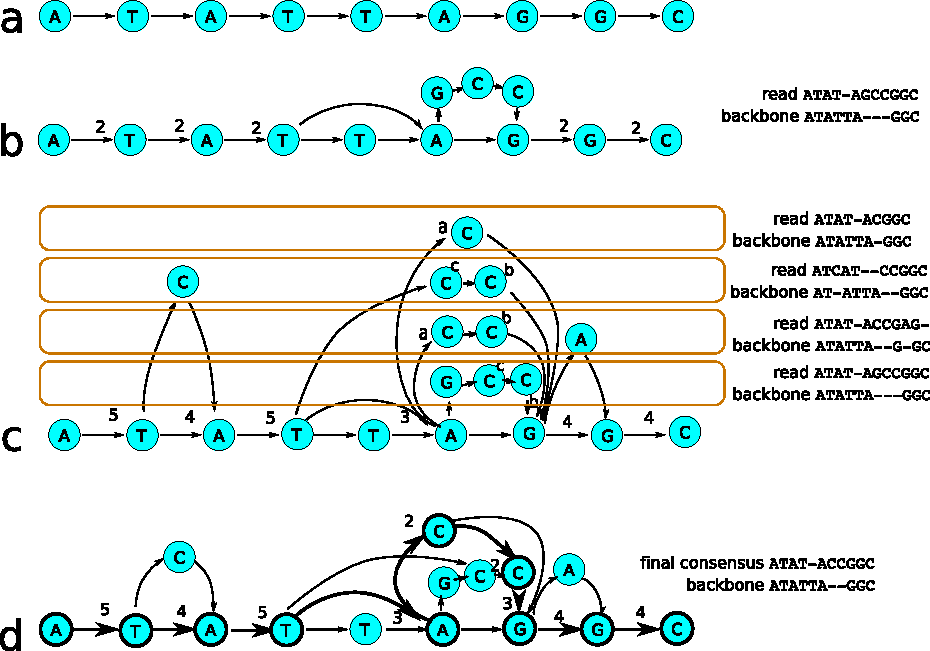
\includegraphics[width=\textwidth]{state_of_the_art/images/POA_explain.pdf}
    \caption{A sequence that needed to be corrected was represented by a graph, each base was a node and if a base was followed by another one a directed edge was built. (b) was the representation of sequence \texttt{ATATTAGGC} (called backbone in this figure), (b) We add the result of alignment of one read in the graph. The number upper than edge was her weigth if and edge exist in some 3 alignment her weight was egal to 3, (c) We add all other alignments in the graph, (d) the bold path was chosen as the correct path because it was supported by more alignments. This figure was originally present in Supplementary material of \hgap \cite{hgap}}
    \label{sota:fig:canu:correction}
\end{figure}

\subsection{Trimming}

The trimming step will remove the parts of the reads that are not supported by the other reads, see Figure \ref{sota:fig:canu:trimming}. For each read we will analyze its coverage curve and remove the parts of the read that are not sufficiently covered (by default this value is set to 1). For trimming, \canu uses a homemade tool. 


\begin{figure}[ht]
    \centering
    \subfile{state_of_the_art/tikz/trimming.tex}
    \caption{The black line is a read, the \canu trimming step keeps only the blue part of read $R_0$, part covered by other read.}
    \label{sota:fig:canu:trimming}
\end{figure}

\subsection{Assembly}

The assembly step in \canu pipeline is based on the \OLC paradigm (see Section \ref{intro:subsec:OLC} for a definition of \OLC), with some specificities. \canu builds a Best Overlap Graph (BOG) for each non-contained read only two overlaps are kept in the graph, the best overlap for each read extremity, in \canu the best overlap was the longest overlap. Use of a BOG instead of a classic \OLC graph is an aggressive strategy, in BOG we cannot observe a transitive edge and the number of edges is bound by the number of node. We avoid a cleaning step and reduce the memory impact of the graph. Once this graph construction step is performed, a clean step is run, removing tips and little bubbles (see Section \ref{intro:subsubsec:bubble_tips}).

This BOG was used as a scaffold to generate assembly. By remapping read against this scaffold, \canu tries to detect repetition, larger than read not show in BOG as loop. This mapping is used after to build the consensus sequence of contigs. Each simple path in BOG was used to build a contig. 

By remapping reads on the BOG \canu can build a consensus and detect repetitions not observed in the graph. BOG was an aggressive strategy to avoid transitive edge and reduce graph size but they can mask an edge denote a repetition this check was required to.

\begin{figure}[ht]
    \centering
    \subfile{state_of_the_art/tikz/BOG_remapping.tex}
    \caption{Black arrow line was the path chosen by \canu, the other line was a read mapped against this path, the blue box indicates a repeat region. In case \texttt{A} the purple read spans all the repetition and indicates that the path chosen by \canu was the good one. In case \texttt{B} no read spans the repetition and the purple read have non-congruent overlaps between the red and blue reads, so \canu needs to break the path in order not to create a misassembly}
    \label{sota:fig:canu:remapping}
\end{figure}

\section{Pipeline without correction \miniasm} \label{section:sota:miniasm}

\minimap and \miniasm was an assembly pipeline proposed in \cite{miniasm_minimap} and \cite{minimap2}, the main purpose of this pipeline is to demonstrate that we can perform a long read assembly without correct long read before.

The miniasm pipeline is more simple than the canu pipeline because it does not incorporate correction and consensus building. It is made of steps:
\begin{itemize}
    \item overlap search, performed by minimap
    \item trimming, by miniasm
    \item graph construction 
    \item graph cleaning
    \item contig generation
\end{itemize}


\subsection{\minimap} \label{subsec:sota:miniasm:minimap}

The main idea with \minimap (similar to \mhap) is that we can represent a read as a set of minimal kmer, and if two reads share the same succession of minimal kmer we can suppose these two reads share an overlap.

A minimal kmer is, for a set of consecutive kmer, the one that minimizes its score. The score function was the same during the whole analysis and for the same set of consecutive kmer, the same kmer was the minimizer. Moreover, a kmer can be the minimizer for several consecutive sets of kmer if no kmer with a lower score comes in the window. 

\begin{figure}[ht]
    \centering
    \subfile{state_of_the_art/tikz/minimizer.tex}
    \caption{The red kmer has the lowest score of the red window, so it is the minimizer of this window. But when window slice on the blue kmer this one has a lower score, the blue kmer become the minimizer of this window.}
    \label{sota:fig:miniasm:minimizer}
\end{figure}

The minimal \kmer can represent many other reads, this technique can be compared to a loosly compression.

\minimap builds an index in which each minimizer is associated to the reads where a minimizer is present and the position of the minimizer in the reads.

With this index \minimap can collect the positions of similar minimizers between two reads. With this collection of positions \minimap looks for the largest co-linear match, a succession of similar minimizers in each read with coherent position, same order of minimizer and similar distance between each minimizer. Figure \ref{sota:fig:miniasm:mapping} shows an overview of an overlap of two reads in \minimap.

\begin{figure}[ht]
    \centering
    \subfile{state_of_the_art/tikz/minimap.tex}
    \caption{$Read_A$ and $Read_B$ are represented by black arrows. The common minimizers of $Read_A$ and $Read_B$ are represented by blue and red arrows respectively. The green arrows are a co-linear chain, the purple arrows another co-linear chain, the black arrows do not participate in a co-linear chain. The longest colinear chain is the green one. The end of $Read_A$ probably overlaps with the beginning of $Read_B$.}
    \label{sota:fig:miniasm:mapping}
\end{figure}

\minimap reports overlap where the number of matches is sufficient (greater than a threshold) and  total length of putative overlap is sufficient. 

\subsection{\miniasm}

\miniasm did not perform correction but it did not take all the information from reads and overlaps either; a filtering operation was performed.

For each read \miniasm performs coverage analysis of reads based on mappings identified by \minimap, by default only the longest part of reads with a coverage greater than three is kept. \minimap reports for each read, read length, position of first and last kmer, number of bases in kmer exact match, and a mapping quality and some option fields in SAM-like format can be present too.

\begin{figure}[ht]
    \centering
    \subfile{state_of_the_art/tikz/miniasm_overlap.tex}
    \caption{\miniasm classifies overlaps in three types of dovetail, internal match and containment overlap. The dark grey region corresponds to the part of the read between the first and last minimizer. The light grey region is called the overhang region, it is out of minimizer range. If overhang is large compared to the overlap region, we can suspect the overlap is not a true overlap.}
    \label{sota:fig:miniasm:ovl_classification}
\end{figure}

Each overlap was classified in three categories, in order to keep only true end-to-end overlaps to build the \OLC and filter out containment reads:
\begin{itemize}
    \item internal match, this type of overlap probably corresponds to a repetition smaller than reads length
    \item containment, a read of this overlap was contains in the other read it's same sequence
    \item dovetail, it is an end-to-end overlap
\end{itemize}
Figure \ref{sota:fig:miniasm:ovl_classification} shows examples of these overlaps. Containment read was removed, only dovetail overlap was used to build the overlap graph. Tips, small bubbles and transitive edges were removed after this step. \miniasm takes each simple path and concatenates substring of read between the beginning and the first position of overlap.

\miniasm was design to work on uncorrected reads and did not perform a consensus step, so contigs generated by \miniasm contains many errors and cannot be used directly. We can run the \minimap \miniasm pipeline with corrected read and a polishing tool on contigs generated by \miniasm.

Very recently, another assembly tool \toolsname{Ra}\cite{Ra} was a created to replace \miniasm in \minimap \miniasm pipeline. \toolsname{Ra} uses an analysis of coverage curve of each read to trim not supported region like \miniasm but they include the detection of chimera and repeat region. Overlaps on region marked as repeat are marked in a string graph and not trusted. \toolsname{Ra} performs a real consensus step and runs many polishing step with \toolsname{Racon}. According to the authors and to another study\cite{long_read_assembler_comparison}, Ra performs good assembly on bacteria and plant genome assembly the overlap step still can be optimize in term of memory usage and computation time.

\section{\DBG like long reads assembly approach} \label{section:sota:wtdbg}

\DBG tools try to speed up assembly by simplifying the overlap search step. This method was proposed in \toolsname{EULER} \cite{eulerian_approach}.

This approach is based on a DeBruijn Graph (or \DBG). For an alphabet with $n$ symbols, a \DBG represents each word of length $k$ as a node and builds a directed edge if nodes share $k - 1$ symbols at their extremities. For example, in Figure \ref{intro:fig:dbg:graph}, node \texttt{ATCG} and \texttt{TCGG} share \texttt{TCG}. A word of length $k$ is called a \kmer.

In assembly problems, $n = 4$ (${A, C, T, G}$), and we can choose a value of k between 1 and the read length. In practice, the size is often smaller than the size of a read. The choice of the right values for k, depending on the use that we will have of the \DBG, could be the subject for a whole thesis.

To build the \DBG we chose a value for $k$ and added all \kmer present in reads in the \DBG. The \DBG used in assembly contains only the \kmer present in the dataset, not all possible \kmer, and edges can be only edges that are present in the dataset or all possible edges.

\begin{figure}[ht]
    \center
    \subfile{introduction/tikz/debruijn_graph.tex}
    \caption{We have a dataset of 4 reads with length equal to 7, we choose a value equal to 4, kmer was present under each read. A \DBG built from this kmer set is present under kmer, each node is a kmer and if a word shares $k - 1$ symbol at its end with $k - 1$ symbols at the beginning of another node, we build a directed edge. This \DBG contains a cycle. This cycle probably matches a repetition in the original sequence.}
    \label{intro:fig:dbg:graph}
\end{figure}

Like \OLC we can detect repetition by inspecting the number of successors of a node. Figure \ref{intro:fig:dbg:graph} presents a \DBG with a repetition. After building the \DBG we can follow the simple path to rebuild the original sequence.

With the \DBG strategy we did not compute overlaps between reads, but the word length in the graph was shorter. And all repetitions with a size greater than $k$ create a cycle in the graph and fragment the assembly.

Moreover the overlap between words in \DBG must exact (without error) and with a fixed length ($k - 1$). These two constraints are particularly problematic when the reads contain a lot of errors or when the coverage of the region is low.

The \DBG approach was used successfuly for short-read assembly. We can mention the tools \toolsname{Spades} \cite{spades}, \toolsname{Minia} \cite{minia} and \toolsname{Megahit}\cite{megahit} but these methods are not very efficient for long reads assembly:
\begin{itemize}
    \item reads contain a high error rate and therefore finding error-free kmers was hard, these errors can lead to expand the size of the graph and or mis-connection between part of graph.
    \item the size of the kmer was generally less than 100 bases and it was difficult to manage larger without using of a lot of memory.
\end{itemize}

If we use \DBG naively for long read assembly, we can miss the main advantage of long-reads: their length.

\flye and \wtdbg use the \DBG approach with some modifications to adapt the idea to long-read assembly. \flye creates a A-Bruijn Graph (\abreviation{ABG}), in which an edge does not signal an overlap with a k-1 length between nodes but the overlap can be shorter. In \wtdbg method kmer are replaced with k-bin where a bin is a substring (256 bases of length by default) of reads, and is generated between k-bin if they are successive in a read.

\subsection{\flye}

\flye\cite{Flye} was based on \abruijn\cite{abruijn} assembly tools. \abruijn did not use a \DBG but a similar concept a \abreviation{ABG}, instead of using a set of kmers as nodes, \abreviation{ABG} uses a set of chosen kmers, instead of building an edge between each kmer they share a k-1 overlap, they build an edge with a weight equal to the distance of kmer in the read without creating a transitive edge.

To build the chosen \kmers set, \abruijn selects kmers present many times in the dataset. These kmers are called in many tools \textit{solid} \kmers \jsv{citer le papier qui introduit la notion de solid kmer} \pim{Sa existe ? demander a Rayan}. The more present a \kmer is in the dataset, the more confident you can be that the \kmer does not contain a sequencing error. If the genome coverage is 40x we can hope see \kmer, not include in a repetition, 40 times. Because when we sequence at 40x, we do not actually read each base 40 times; and when a sequence error appears, we lose an occurrence of the kmers where this base was present. Choosing the number of times a kmer has to be present in the dataset to be \textit{solid} was a difficult task.

This modification helps to clean sequencing error, but reduces the set of kmer fragments the \DBG graphs. This is why \abreviation{ABG} creates edges not only when kmers share a k-1 overlap. 

During the \abreviation{ABG} construction, \abruijn stores which read generates which graph path. This structure was useful to find quick overlaps between reads. Reads participating in the same path of \abreviation{ABG} probably have the same sequence, so they probably share an overlap. To build contigs, \abruijn takes a read found all overlap with help of \abreviation{ABG}. If this local overlap graph didn't denote a fork (we have one read without successor and all reads have path in the local overlap graph to this read), \abruijn extend the contig.

\abruijn can be roughly summed up as mix of all the assembly strategies, using \DBG to find overlaps between reads, building contigs by extension as with \textit{greedy} method but using \OLC to make sure they do not integrate a repetition and a potential missassembly in contigs.

\flye was built on top of \abruijn. After the \abruijn assembly, \flye looks for self-alignments in the assembly. If the extremity of a contig are similar they are tag as repetition. \flye builds a repetition graph, where repetition extremity as node and a edge was build when to repetition extremity was link in a contig. \flye uses coverage information to take a clue on contig succession over untangle repetition. By analysing the topology of repetition graphs, \flye can find a unique traversal path to explain all repetitions and find the genomic order of a contig.

\subsection{\wtdbg}

\wtdbg \cite{wtdbg2}  uses a \DBG approch to solve long-read assembly. It is not really a \DBG, but a "Fuzzy-Brujin graph" (\abreviation{FDBG}) firstly define in this paper. To build this graph, \wtdbg splits a read in a bin with a fixed size (256 base pairs) and stores the kmer present in each bin in a hash table.
To find the overlap between reads, wtdg2 uses a hash table to compare the kmer compositions between each read and performs an exact alignment between each bin of reads.

After this alignment step, \wtdbg only keeps in memory which bin is aligned to which bin, and it builds k-bins. Each k-bin is a sequence of k successive bin in a read. \wtdbg can infer if two k-bins overlap if one bin in this two k-bins shares an ovelap.

A group of k-bins are a node of \abreviation{FDBG}. \wtdbg builds an edge between two nodes if a k-bins in each node are successive in a read, after some cleaning step (pops bubbles, tips cleaning) \wtdbg builds a consensus sequence with each simple path in \abreviation{FDBG}.

\section{New long read assembly method}

Very recently, two assembly tools have been presented that focus on the ability to produce good long read assembly with a very low cost in computation time and memory use.

\subsection{Peregrine}

\newcommand{\shimmer}{\toolsname{SHIMMER}}

\peregrine \cite{Peregrine} uses the \shimmer overlapper. \shimmer extends idea of minimizer (introduced in Section \ref{subsec:sota:miniasm:minimap}), by creating a minimizer of minimizers. A minimizer can represent a set of minimizers. These minimizers representing a set of kmer, we can have many layers of minimizers, each layer reducing the size of the minimizer set and the space of search to find similarities between reads.

The layer-0 of minimizers was a basic minmizer process, like \minimap. After this step, \shimmer selects minimizer they participate to the layer-1, it uses a reduction factor, for a reduction factor $x$, $x$ minimizers are represented by the minimal minimizer of this set. This process can be repeated with many layers. When it chooses the minimizer of $layer_n$ minimizer of $layer_{n-1}$, \shimmer pays attention to the distance between each $layer_n$ minimizer to be sure they represent a distinct part of the read. \shimmer by default uses three layers of minimizing this value, reduces the number of minimizers needed to be compare to found similarity, without increasing the number of missed overlaps (value found empirically).

After this indexing step, \shimmer brings together reads that share many last layer minimizers and performs a classic alignment to confirm overlap between reads. After this step, \peregrine runs a classic \OLC strategy to perform assembly.

\shimmer overlapping tools can be used to perform a mapping of read against contig or genome. After this remapping a polishing step was performed, without taking into account heterozygosity.

\peregrine was actually tested only on Circular Consensus (CCS) Pacbio data. Reads were sequenced multiple times and a consensus was performed on all this sequencing. This technique reduces the read length but reduces the error level of sequencing too. Finding overlaps between reads with less error was easier and faster. Methods created by \peregrine tools by reducing the minimizer space of search speed up the search for overlaps, but it was tested on low error rate long reads, even if the error rates of long reads try to decrease, will they decrease sufficiently for this method to maintain a good sensitivity. \peregrine needs to be validated on other types of data before its method can be generalized.

\subsection{Shasta}

\newcommand{\shasta}{\toolsname{Shasta}}

\shasta is a recently published assembly tools that was used to assemble Nanopore data of eleven human genomes \cite{Shasta}.

\shasta uses read-length representation of reads. Read-length representation is a loss-less compression method for text that contains a large repetition of the same character. For example, the sequence \texttt{ACCTTTGAA}, was represented by two strings $Sb$ \texttt{A C T G A} and $St$ \texttt{1 2 3 1 2}. To reconstruct the original sequence, we repeat $St_i$ time the $Sb_i$ letter.

This representation was interesting for long-reads data, because DNA contains sometimes the same character repetition (called an homopolymer) and long-reads often make errors in homopolymer. Read-length representation by squashing this region can avoid this type of error and facilitates the alignment of long-reads.

To perform read overlapping, \shasta did not use a minimizer approach but something very close, the $Sb$ string of read was split in kmer and some kmer were selected randomly, and called markers. The set of markers was the same for all data set. Reads was now represented by a succession of markers: it is a lossly compression.

Before looking for a colinear match of marker, in order to select reads with a higher match probability, \shasta computes a modification of the MiniHash Jaccard estimation (see Section \ref{subsec:sota:canu:overlapping}) to avoid the bias created by the difference of length between reads.

To perform assembly \shasta creates a marker graph. It is something similar to \DBG, where kmer was a marker and an edge was built between two markers if a read contained this succession of markers. Each edge was weighted by the number of reads that contained this succession. After a cleaning step of marker graph (removing transitive edges, tips and bubbles), a path in marker graph was selected and reads participate to building of edge of this path was used to build a consensus sequence of contigs.

\shasta contains many interesting ideas and the authors plan improvements for heterozygosity detection, resolution and performance improvement.

\section{Chapter Conclusion}

Long read assembly is an active field of research, many tools are created each year and long read assembly tools are used to improve genome and build draft genome.

To perform overlap detection, a majority of tools use k-mer to find reads with a high similarity and avoid all-versus-all overlapping search. To further reduce the space search, some tools use filtering based on minimizing: we keep the kmer with the lowest score, this score can be based on information contained in the dataset or be determined by an arbitrary function. The choice of k-mer size, filtering method and minimizing function, can have a great impact on result of each tool.

The \OLC approach has proven its effectiveness in assembling third generation reads. Several modifications have been made to support these new reads but efforts are mainly focused on reducing the computation time of memory usage. These modifications lead to hybrid \OLC algorithm with \DBG and Greedy, (cf \flye and \wtdbg) idea. But the step that takes the most time and memory is not the graph construction and contig construction, it is the search for overlap and the correction.

This is not the only the challenge that needs to be addressed. Many assembly steps have a considerable cost in computation time and memory use. One challange, for example, would be to be able to conduct an overlap search with high precision and recall without excessive cost in computation time and memory use \cite{bench_ovl}.

The only assembly that tried to take heterozygosity into account was \toolsname{FALCON} – in future the, \shasta will do it as well –, by making the difference between a sequencing error and a natural variant or heterozygosity. To get heterozygosity and variant phased or genome graph after assembly would be interesting. But the tools to extract all this information from a read do not exist yet.

Another step of assembly improvement was increase the contiguity, assembly tools by reducing the information to reduce computation time and memory use can have an impact on assembly quality. Correction of long-read can by trimming insufficient covered data can increase the size of coverage gap.
By come back to all read information or use overlap found by another tools, help to solve assembly trouble, created by heuristic in assembly and correction tools. The next chapter focuses on this point.


\onlyinsubfile{
\bibliographystyle{plainnat}
\bibliography{main}
\addcontentsline{toc}{chapter}{Bibliography}
}

\end{document}